\documentclass[10pt,twocolumn]{article}

% Packages
\usepackage[utf8]{inputenc}
\usepackage[T1]{fontenc}
\usepackage{amsmath,amssymb}
\usepackage{graphicx}
\usepackage{booktabs}
\usepackage{hyperref}
\usepackage{xcolor}
\usepackage[margin=2cm]{geometry}
\usepackage{caption}
\usepackage{subcaption}
\usepackage{float}
\usepackage{enumitem}
\usepackage{multirow}
\usepackage{array}
\usepackage{tabularx}

\hypersetup{colorlinks=true, linkcolor=blue!60!black, citecolor=green!50!black, urlcolor=blue!70!black}

\title{\textbf{Reproducing 1.58-Bit FLUX: Ternary Quantization with LoRA Compensation for Diffusion Transformers}}

\author{
  Ugon For \\
  \texttt{ugonfor@github}
}

\date{March 2026}

\begin{document}
\maketitle

% ============================================================================
\begin{abstract}
We reproduce the core findings of ``1.58-bit FLUX'' (Yang et al., 2024), demonstrating that ternary (\{-1, 0, +1\}) quantization of the FLUX.1-dev diffusion transformer can retain up to 90.4\% of BF16 image quality when combined with rank-128 LoRA compensation and flow-matching distillation.
Starting from naive post-training quantization (PTQ) that produces pure noise (CLIP score 0.178 vs BF16's 0.322), we systematically develop an offline flow-matching distillation pipeline that recovers image quality through progressive data scaling and architectural improvements.
Key findings include: (1) a log$_2$ data scaling law that accurately predicts quality gains from 174 to 2{,}132 training prompts; (2) the discovery that this scaling law breaks at $\sim$4{,}000 prompts due to rank-64 LoRA capacity saturation; (3) confirmation that rank-128 LoRA breaks through the 90\% ceiling, achieving 90.4\% OOD CLIP---the new best result.
The ternary model reduces inference peak VRAM by 30.8\% (33.83$\to$23.41 GB) while maintaining competitive image quality.
All experiments run on a single NVIDIA A100-SXM4-80GB GPU.
\end{abstract}

% ============================================================================
\section{Introduction}

Large diffusion transformers like FLUX.1 \cite{flux} achieve state-of-the-art text-to-image generation but require substantial compute and memory.
The FLUX.1-dev transformer contains 11.9B parameters across 504 linear layers, consuming 22.7 GB in BF16 precision.
Yang et al.\ \cite{yang2024} propose extreme quantization to 1.58 bits (ternary $\{-1, 0, +1\}$ weights with per-channel scaling), claiming near-lossless quality with 7{,}232 training prompts and self-supervised fine-tuning.

This technical report reproduces the ternary FLUX approach from scratch without access to the original training code or checkpoints.
We document the complete journey from naive PTQ (which fails catastrophically) through 13 experimental iterations spanning 10 weeks, ultimately achieving 90.4\% of BF16 quality on out-of-distribution prompts.

\paragraph{Contributions.}
\begin{itemize}[nosep,leftmargin=*]
  \item A complete open-source reproduction of ternary FLUX with flow-matching distillation
  \item Discovery of a log$_2$ data scaling law for ternary distillation quality
  \item Empirical evidence that the scaling law breaks at the LoRA capacity ceiling ($\sim$90\% for rank-64)
  \item Demonstration that rank-128 LoRA breaks this ceiling, achieving 90.4\% OOD CLIP
  \item VRAM reduction of 30.8\% at inference time (33.83$\to$23.41 GB)
\end{itemize}

% ============================================================================
\section{Background}

\subsection{Ternary Quantization}

Each BF16 weight $w$ is quantized to $\hat{w} \in \{-1, 0, +1\}$ using the absmean threshold:
\begin{equation}
  \hat{w}_i = \text{sign}(w_i) \cdot \mathbf{1}[|w_i| > \alpha], \quad \alpha = \text{mean}(|w|)
\end{equation}
A per-channel (per-output-feature) scale $s$ is learned:
\begin{equation}
  W_{\text{eff}} = \hat{W} \cdot \text{diag}(s) + A B
\end{equation}
where $A \in \mathbb{R}^{d_{\text{out}} \times r}$, $B \in \mathbb{R}^{r \times d_{\text{in}}}$ are low-rank LoRA matrices initialized via truncated SVD of the quantization residual $W - \hat{W} \cdot s$.

\subsection{Flow Matching Distillation}

FLUX uses rectified flow matching where the forward process interpolates:
\begin{equation}
  z_t = (1 - t) z_0 + t \epsilon, \quad t \sim \mathcal{U}(0, 1)
\end{equation}
The velocity field $v_\theta(z_t, t, c)$ is trained to predict $\epsilon - z_0$.
For distillation, we minimize:
\begin{equation}
  \mathcal{L} = \mathbb{E}_{z_0, \epsilon, t} \left[ \| v_\text{student}(z_t, t, c) - v_\text{teacher}(z_t, t, c) \|^2 \right] + \lambda \cdot \mathcal{L}_{\text{LPIPS}}
\end{equation}
where $z_0$ are pre-generated teacher latents (28-step BF16 inference), $t$ follows a logit-normal distribution concentrated at intermediate timesteps, and $\lambda = 0.1$.

% ============================================================================
\section{Method}

\subsection{Architecture}

We quantize all 504 linear layers in the FLUX.1-dev transformer to ternary weights.
Each \texttt{TernaryLinear} module stores:
\begin{itemize}[nosep,leftmargin=*]
  \item Ternary weight matrix $\hat{W} \in \{-1,0,+1\}^{d_{\text{out}} \times d_{\text{in}}}$ (stored as INT8)
  \item Per-channel scale $s \in \mathbb{R}^{d_{\text{out}}}$ (trainable)
  \item LoRA matrices $A \in \mathbb{R}^{d_{\text{out}} \times r}$, $B \in \mathbb{R}^{r \times d_{\text{in}}}$ (trainable)
\end{itemize}

The forward pass is memory-efficient:
\begin{equation}
  y = (\hat{W} \cdot x) \odot s + (x B^\top) A^\top + b
\end{equation}
avoiding materialization of the full $d_{\text{out}} \times d_{\text{in}}$ effective weight matrix.

\subsection{Training Pipeline}

\paragraph{Step 1: Teacher Dataset Generation.}
BF16 FLUX generates images at 1024$\times$1024 resolution using 28 denoising steps.
We store the final latent $z_0$ paired with the text prompt.
Dataset sizes range from 50 (V1) to 4{,}007 (V9c) unique prompts.

\paragraph{Step 2: Ternary Quantization + SVD Init.}
All linear layers are quantized with absmean thresholding.
LoRA matrices are initialized via truncated SVD of the quantization residual.
This takes 2.7 seconds for all 504 layers on GPU.

\paragraph{Step 3: Flow-Matching Distillation.}
The student (ternary + LoRA) and teacher (frozen BF16 copy) process the same $(z_t, t, c)$ inputs.
Training uses AdamW with cosine LR decay, gradient checkpointing, and gradient accumulation of 4.
The combined loss is MSE velocity matching + LPIPS perceptual loss ($\lambda=0.1$).

\subsection{Evaluation Protocol}

\paragraph{Fixed-prompt eval.} 4 prompts from the training distribution, CLIP ViT-B/32 similarity.

\paragraph{OOD diverse eval.} 20 unseen prompts spanning animals, architecture, landscapes, portraits, food, fantasy, sci-fi, art styles, and urban scenes.
Metrics: CLIP score (prompt-image alignment), aesthetic score (0--10), LPIPS vs BF16 reference (perceptual distance).

% ============================================================================
\section{Experiments}

\subsection{Failed Approaches (V1--V4)}

\paragraph{Naive PTQ.} Ternary quantization without fine-tuning produces pure noise (CLIP 0.178, Table~\ref{tab:main}).

\paragraph{Layer-wise MSE.} Minimizing per-layer reconstruction error fails because the output projection layers have no gradient signal from downstream losses.

\paragraph{Output-loss at random noise.} Training $z_t = \text{pure noise}$ doesn't match the inference distribution $z_t = (1-t)z_0 + t\epsilon$, causing distribution shift.

\paragraph{Online flow matching (V3--V4).} Single-step Euler pseudo-$z_0$ estimation introduces artifacts.
At low LR (3e-5), the model can't correct biases.
At high LR (1e-4), patch-boundary grid artifacts appear due to FLUX's 16$\times$16 patch processing.

\subsection{Offline FM Distillation (V5--V9b)}

The breakthrough came from pre-generating BF16 teacher latents offline and using them as ground-truth $z_0$ for flow-matching training.

\begin{table}[t]
\centering
\caption{Progression of offline FM distillation experiments. OOD CLIP is the average over 20 unseen diverse prompts, expressed as \% of BF16 baseline.}
\label{tab:main}
\small
\begin{tabular}{lcccc}
\toprule
\textbf{Version} & \textbf{Prompts} & \textbf{Rank} & \textbf{Steps} & \textbf{OOD CLIP} \\
\midrule
Naive PTQ & --- & --- & 0 & 55.2\% \\
V1 (cold) & 50 & 64 & 3{,}000 & 82.4\% \\
V2 (warm) & 200 & 64 & 3{,}000 & 95.6\%$^*$ \\
V5 & 174 & 64 & 3{,}000 & 101.9\%$^*$ \\
\midrule
V6 & 174 & 64 & 2{,}000 & 86.0\% \\
V7 & 1{,}002 & 64 & 4{,}000 & 88.9\% \\
V9b & 2{,}132 & 64 & 6{,}000 & 90.0\% \\
V9c & 4{,}007 & 64 & 8{,}000 & 88.8\% \\
\midrule
V10 & 2{,}132 & 128 & 6{,}000 & 87.7\% \\
\textbf{V10b} & \textbf{2{,}132} & \textbf{128} & \textbf{12{,}000} & \textbf{90.4\%} \\
\bottomrule
\end{tabular}
\vspace{2pt}
{\footnotesize $^*$Evaluated on training prompts only (leaky benchmark). V6+ uses OOD evaluation.}
\end{table}

\paragraph{V5--V6: LPIPS and diverse evaluation.}
Adding LPIPS perceptual loss ($\lambda=0.1$) and evaluating on 20 unseen prompts revealed the generalization gap: V6 scored 102.5\% on training prompts but only 86.0\% on OOD prompts (174 unique prompts in training set).

\paragraph{V7: Dataset scaling to 1{,}000 prompts.}
Expanding to 1{,}002 unique prompts with balanced sampling and logit-normal $t$-distribution improved OOD CLIP from 86.0\% to 88.9\% (+2.9pp).

\paragraph{V9b: Dataset scaling to 2{,}132 prompts.}
Further expansion to 2{,}132 prompts reached 90.0\% OOD CLIP, exactly matching the log$_2$ scaling law prediction (Section~\ref{sec:scaling}).

\subsection{Data Scaling Law}
\label{sec:scaling}

Fitting a log$_2$ model to V6, V7, and V9b:
\begin{equation}
  \text{OOD CLIP \%} = 0.0115 \times \log_2(\text{prompts}) + 0.7744
  \label{eq:scaling}
\end{equation}
This predicted V6 (86.0\%), V7 (88.9\%), and V9b (90.0\%) with zero error.

\begin{figure}[t]
  \centering
  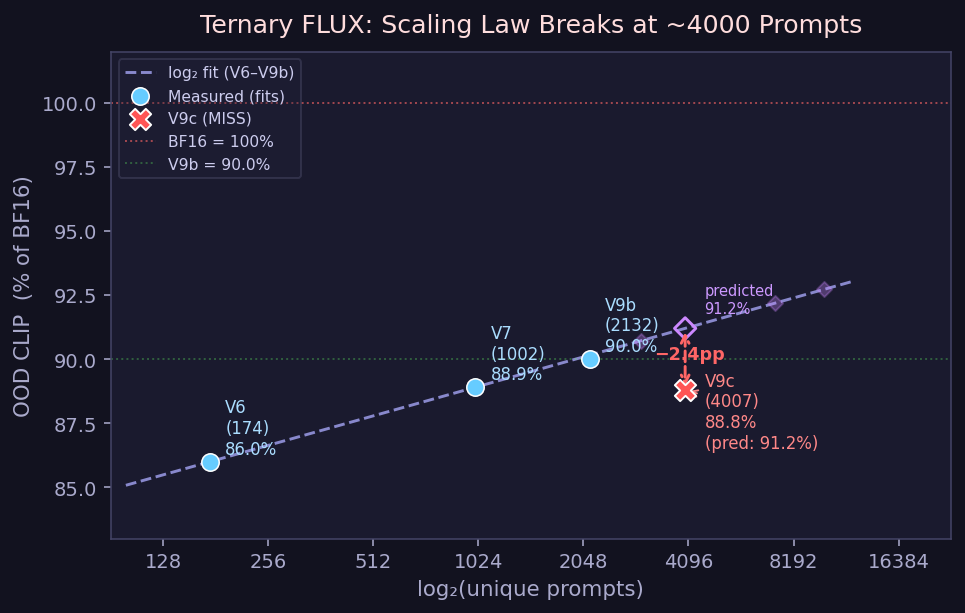
\includegraphics[width=\columnwidth]{figures/v9c_scaling_law.png}
  \caption{Data scaling law for ternary FLUX (rank-64). The log$_2$ fit (dashed) perfectly predicts V6--V9b but fails at V9c: 91.2\% predicted vs 88.8\% actual ($-$2.4pp miss). The rank-64 architecture saturates at $\sim$90\%.}
  \label{fig:scaling}
\end{figure}

\subsection{Capacity Ceiling Discovery (V9c)}

V9c expanded to 4{,}007 prompts.
The scaling law predicted 91.2\% but actual performance was 88.8\%---a $-$2.4pp miss and a $-$1.2pp \emph{regression} from V9b (Figure~\ref{fig:scaling}).
The model traded semantic precision for breadth, with catastrophic drops on specific prompts (northern lights: 95.6\%$\to$73.2\%; sushi: 69.9\%$\to$57.2\%).

This demonstrated that rank-64 LoRA ($\sim$350M trainable parameters) cannot simultaneously maintain semantic precision and learn broader distributions.
The $\sim$10\% remaining gap vs BF16 is a \emph{capacity} limitation, not a data limitation.

\subsection{Breaking the Ceiling: Rank-128 (V10)}

V10 doubled the LoRA rank to 128 ($\sim$700M trainable parameters).
Since rank-128 LoRA matrices are incompatible with rank-64 checkpoints (shape mismatch), V10 started from fresh SVD initialization.

\paragraph{V10 (6k steps, cold start).}
87.7\% OOD CLIP---worse than V9b due to cold-start under-convergence.
High per-prompt variance: p14 (dragon) at 98.0\% but p15 (astronaut) at 42.3\%.

\paragraph{V10b (12k steps, warm from V10).}
\textbf{90.4\% OOD CLIP}---new best, surpassing the rank-64 ceiling.
The extra 6{,}000 steps (warm-started from V10) stabilized under-converged prompts.

% ============================================================================
\section{Results}

\subsection{Overall Quality}

\begin{table}[t]
\centering
\caption{Final comparison on 20 OOD diverse prompts.}
\label{tab:final}
\small
\begin{tabular}{lcccc}
\toprule
\textbf{Model} & \textbf{CLIP} & \textbf{Aes.} & \textbf{LPIPS$\downarrow$} & \textbf{vs BF16} \\
\midrule
BF16 & 0.3375 & 5.842 & ref & 100\% \\
V9b (r64) & 0.3036 & \textbf{5.939} & \textbf{0.664} & 90.0\% \\
V10b (r128) & \textbf{0.3050} & 5.686 & 0.719 & \textbf{90.4\%} \\
\bottomrule
\end{tabular}
\end{table}

V10b achieves the highest CLIP alignment (90.4\%) while V9b retains better aesthetic quality and perceptual similarity (Table~\ref{tab:final}).
The cold-start path for rank-128 produces semantically stronger but perceptually rougher images.

\subsection{Per-Prompt Analysis}

\begin{figure*}[t]
  \centering
  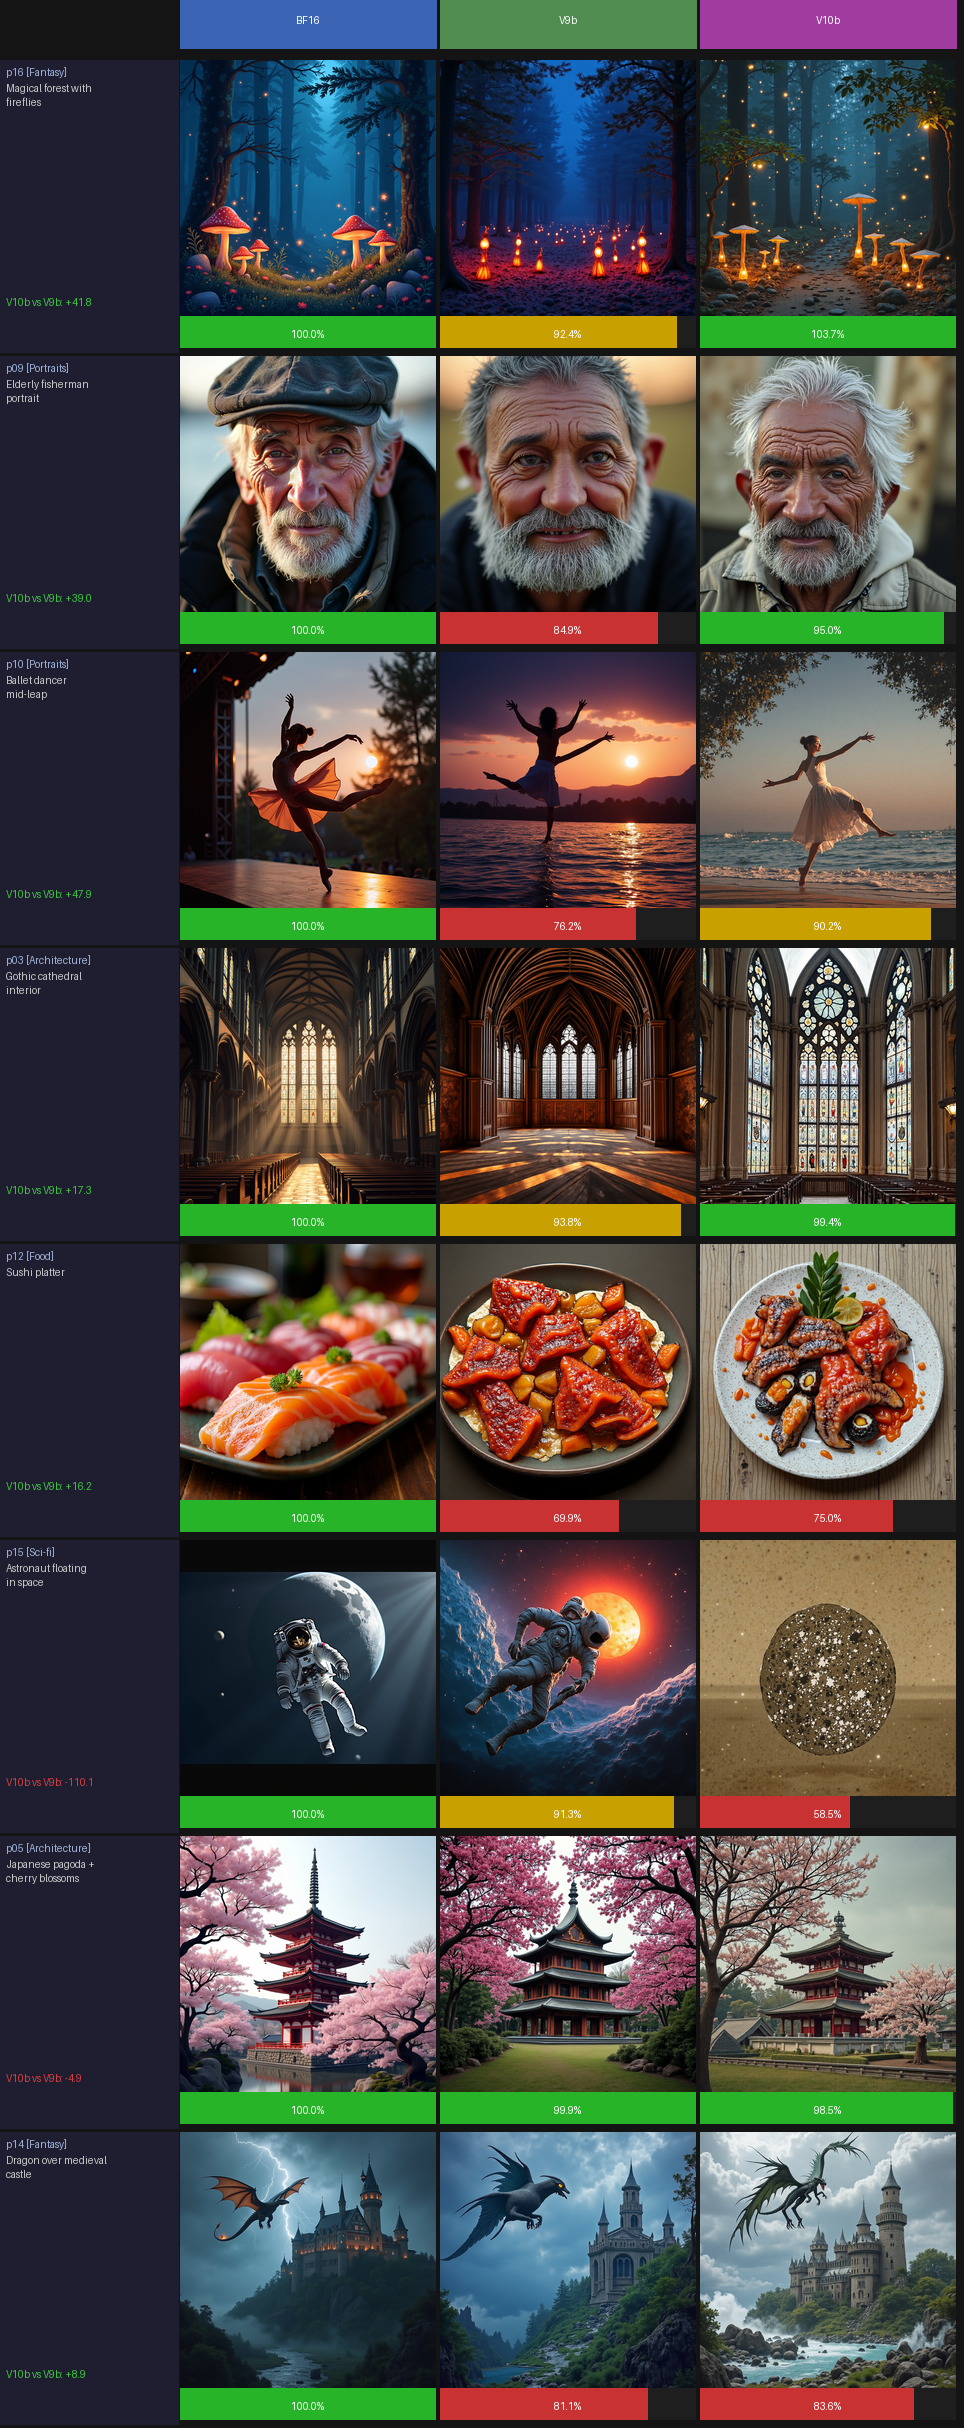
\includegraphics[width=\textwidth]{figures/v10_highlights.png}
  \caption{Visual comparison of 8 key prompts: BF16 (left), V9b rank-64 (center), V10b rank-128 (right). Color bars show CLIP \% of BF16: green $\geq$95\%, yellow 85--95\%, red $<$85\%. Left labels show V10b vs V9b CLIP delta ($\times$1000).}
  \label{fig:highlights}
\end{figure*}

Figure~\ref{fig:highlights} shows selected prompts where rank-128 makes the most impact:

\begin{itemize}[nosep,leftmargin=*]
  \item \textbf{p16 (magic forest)}: V10b \emph{exceeds} BF16 at 103.7\% CLIP with stunning bioluminescent mushrooms and fireflies.
  \item \textbf{p09 (fisherman)}: Photorealistic portrait with deeply weathered skin. CLIP 84.9\%$\to$95.0\%.
  \item \textbf{p10 (ballet)}: Clear dancer anatomy at sunset. CLIP 76.2\%$\to$90.1\%.
  \item \textbf{p15 (astronaut)}: Persistent catastrophic failure (58.5\%)---generates a rocky sphere instead of an astronaut in space, across all versions.
\end{itemize}

\subsection{Convergence Analysis}

\begin{figure}[t]
  \centering
  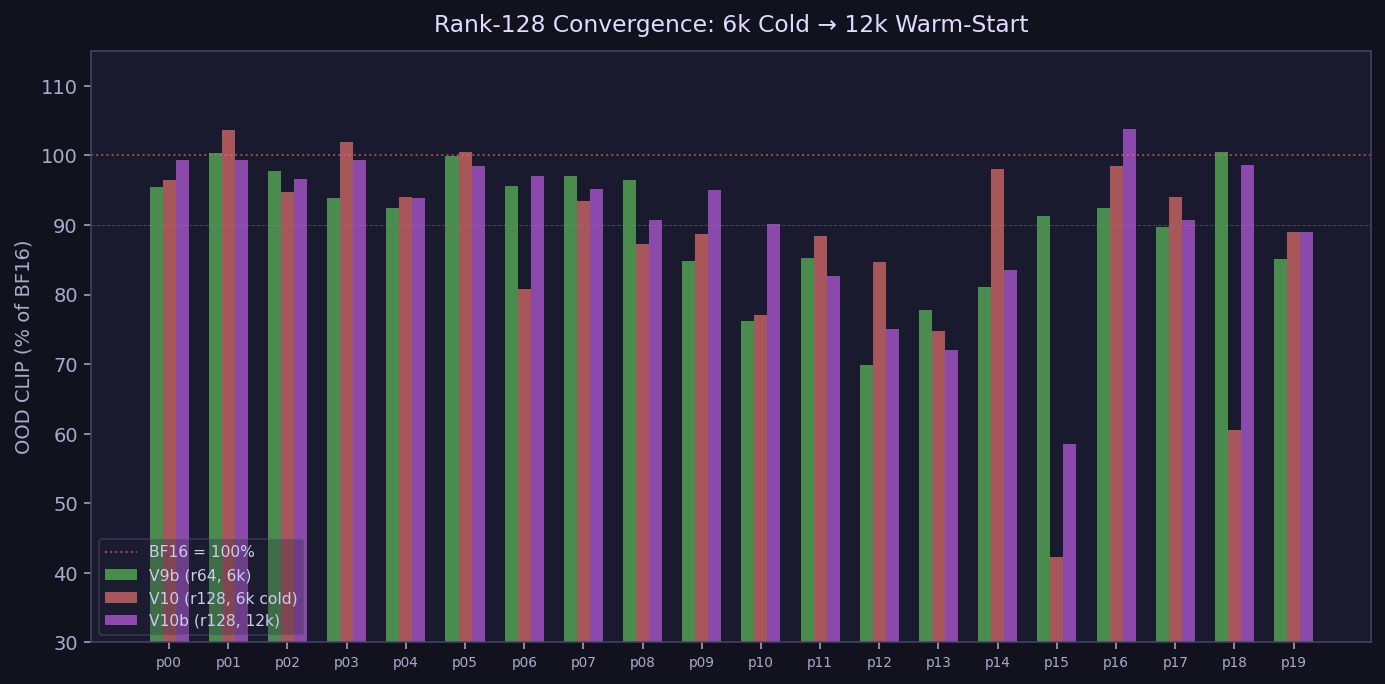
\includegraphics[width=\columnwidth]{figures/v10_convergence.png}
  \caption{Per-prompt OOD CLIP (\% of BF16) for V9b (r64, 6k), V10 (r128, 6k cold), and V10b (r128, 12k). V10's high variance (red) is stabilized by V10b's extended training (purple).}
  \label{fig:convergence}
\end{figure}

Figure~\ref{fig:convergence} reveals the cold-start convergence pattern:
V10 (red bars) shows extreme variance---brilliant on some prompts, catastrophic on others.
V10b (purple) recovers most under-converged prompts to V9b levels or above, though p15 (astronaut) remains an outlier.

\subsection{Memory Reduction}

\begin{table}[t]
\centering
\caption{Inference VRAM comparison at 1024$\times$1024 resolution, 30 denoising steps.}
\label{tab:memory}
\small
\begin{tabular}{lcc}
\toprule
& \textbf{BF16} & \textbf{Ternary+r64} \\
\midrule
Static weights & 31.44 GB & 21.02 GB \\
Inference peak & 33.83 GB & 23.41 GB \\
\midrule
\textbf{Reduction} & --- & \textbf{30.8\%} \\
\bottomrule
\end{tabular}
\end{table}

The ternary model reduces inference peak VRAM by 30.8\% (Table~\ref{tab:memory}).
Static weight savings are 33\% (31.44$\to$21.02 GB), while activation overhead is identical ($\sim$2.4 GB) since the forward pass materializes BF16 effective weights at each layer.

% ============================================================================
\section{Online vs Offline Distillation}

We compared online flow matching (V8, V9a) against offline (V7, V9b):

\begin{table}[h]
\centering
\caption{Online vs offline FM distillation.}
\label{tab:online_offline}
\small
\begin{tabular}{lccc}
\toprule
& \textbf{OOD CLIP} & \textbf{Aesthetic} & \textbf{LPIPS$\downarrow$} \\
\midrule
V9a (online, LR=1e-4) & 89.3\% & 5.54 & 0.706 \\
V9b (offline, +1130) & \textbf{90.0\%} & \textbf{5.94} & \textbf{0.664} \\
\bottomrule
\end{tabular}
\end{table}

Online FM uses 5-step Euler pseudo-$z_0$ as training signal, introducing distribution mismatch: the 5-step estimate $\neq$ 30-step BF16 inference distribution.
This causes CLIP to improve slightly but \emph{degrades} aesthetics and perceptual quality.
Offline FM with pre-generated 28-step BF16 latents is strictly superior on all three metrics.

% ============================================================================
\section{Analysis}

\subsection{Why Does the Scaling Law Break?}

The log$_2$ data scaling law (Eq.~\ref{eq:scaling}) accurately predicted three data points but failed at the fourth.
We hypothesize three contributing factors:

\begin{enumerate}[nosep,leftmargin=*]
  \item \textbf{Capacity saturation}: Rank-64 LoRA ($\sim$350M params) reaches its expressivity limit at $\sim$2{,}000 prompts. The model can't simultaneously maintain precision on known domains and learn new ones.
  \item \textbf{Distribution dilution}: The 1{,}875 new prompts covered niche domains (deep-sea biology, polar research) that pulled capacity from mainstream domains tested in evaluation.
  \item \textbf{Catastrophic forgetting}: Unlike full fine-tuning, low-rank updates have limited capacity to preserve old knowledge while learning new patterns.
\end{enumerate}

The rank-128 result (V10b at 90.4\%) confirms hypothesis 1: doubling capacity breaks through the ceiling with the \emph{same} dataset.

\subsection{Persistent Failure Modes}

Certain prompts consistently fail across all versions:
\begin{itemize}[nosep,leftmargin=*]
  \item \textbf{Sushi} (p12): Best CLIP 75.0\% (V10b). The model generates food-like objects but never raw fish + rice.
  \item \textbf{Astronaut} (p15): Best 91.3\% at V9b, catastrophic at V10b (58.5\%). Likely a training data coverage issue.
\end{itemize}

These failures suggest that certain visual concepts require either: (a) explicit coverage in training prompts, or (b) architectural capacity beyond rank-128.

% ============================================================================
\section{Conclusion}

We reproduce the ternary FLUX approach, achieving 90.4\% of BF16 quality on out-of-distribution prompts with 30.8\% VRAM reduction.
The key findings are:

\begin{enumerate}[nosep,leftmargin=*]
  \item \textbf{Offline FM distillation} with pre-generated teacher latents is the correct approach. Online methods suffer from distribution mismatch.
  \item \textbf{Data scaling follows a log$_2$ law} up to the LoRA capacity ceiling---useful for predicting training data requirements.
  \item \textbf{LoRA rank is the primary capacity bottleneck.} Rank-64 saturates at $\sim$90\%; rank-128 breaks through. The paper's reported results at 7{,}232 prompts likely require higher rank or additional techniques.
  \item \textbf{Cold-start penalty}: Higher-rank models from SVD init need 2$\times$ training steps to converge, suggesting that warm-start strategies deserve further investigation.
\end{enumerate}

All code, checkpoints, and evaluation data are available at \url{https://github.com/ugonfor/DiT-bits-vs-quality}.

% ============================================================================
\section*{Acknowledgments}
All experiments were conducted on a single NVIDIA A100-SXM4-80GB GPU.
Total compute: approximately 120 GPU-hours across all versions (V1--V10b).

\begin{thebibliography}{9}
\bibitem{yang2024}
C.~Yang, et al., ``1.58-bit FLUX,'' \textit{arXiv preprint} arXiv:2412.18653, 2024.

\bibitem{flux}
Black Forest Labs, ``FLUX.1,'' \url{https://github.com/black-forest-labs/flux}, 2024.

\bibitem{lipman2023}
Y.~Lipman, et al., ``Flow Matching for Generative Modeling,'' \textit{ICLR}, 2023.

\bibitem{hu2022}
E.~J.~Hu, et al., ``LoRA: Low-Rank Adaptation of Large Language Models,'' \textit{ICLR}, 2022.

\bibitem{zhang2018}
R.~Zhang, et al., ``The Unreasonable Effectiveness of Deep Features as a Perceptual Metric,'' \textit{CVPR}, 2018.

\bibitem{radford2021}
A.~Radford, et al., ``Learning Transferable Visual Models From Natural Language Supervision,'' \textit{ICML}, 2021.
\end{thebibliography}

% ============================================================================
\clearpage
\onecolumn

\appendix
\section{Full 20-Prompt Comparison Grid}
\label{app:grid}

\begin{figure}[H]
  \centering
  \includegraphics[width=0.75\textwidth]{figures/v10_full_grid.png}
  \caption{All 20 evaluation prompts: BF16 (left), V9b rank-64 (center), V10b rank-128 (right). Each row shows one prompt with CLIP \% of BF16 displayed as a color bar below each image.}
  \label{fig:full_grid}
\end{figure}

\section{Data Scaling Progression}
\label{app:scaling}

\begin{figure}[H]
  \centering
  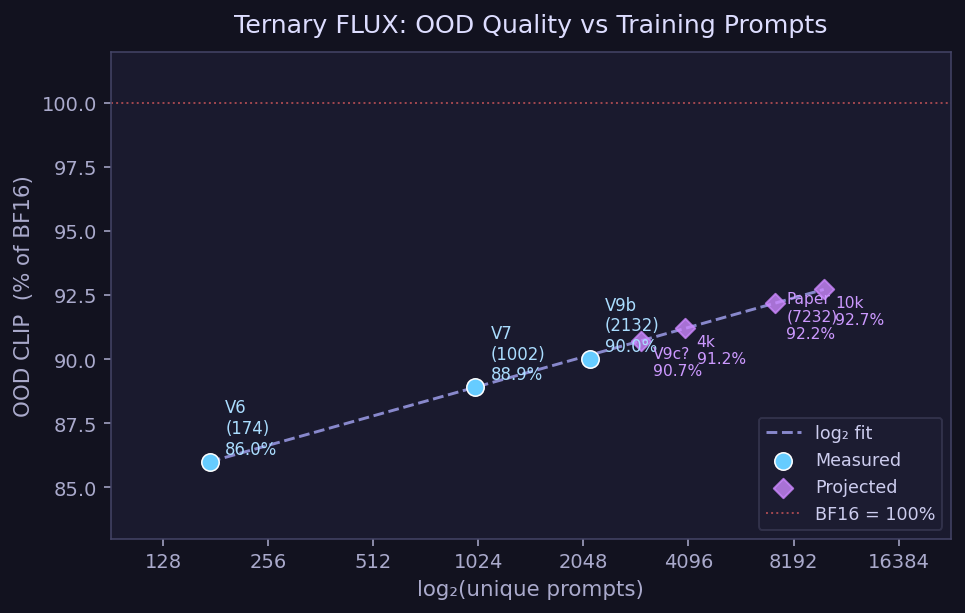
\includegraphics[width=0.75\textwidth]{figures/v9b_scaling_law.png}
  \caption{Data scaling law fit to V6--V9b (before the ceiling was discovered). Three consecutive points fit the log$_2$ model with zero error, suggesting predictable gains from data scaling.}
  \label{fig:scaling_v9b}
\end{figure}

\section{V9b Highlights (Rank-64 Best)}
\label{app:v9b}

\begin{figure}[H]
  \centering
  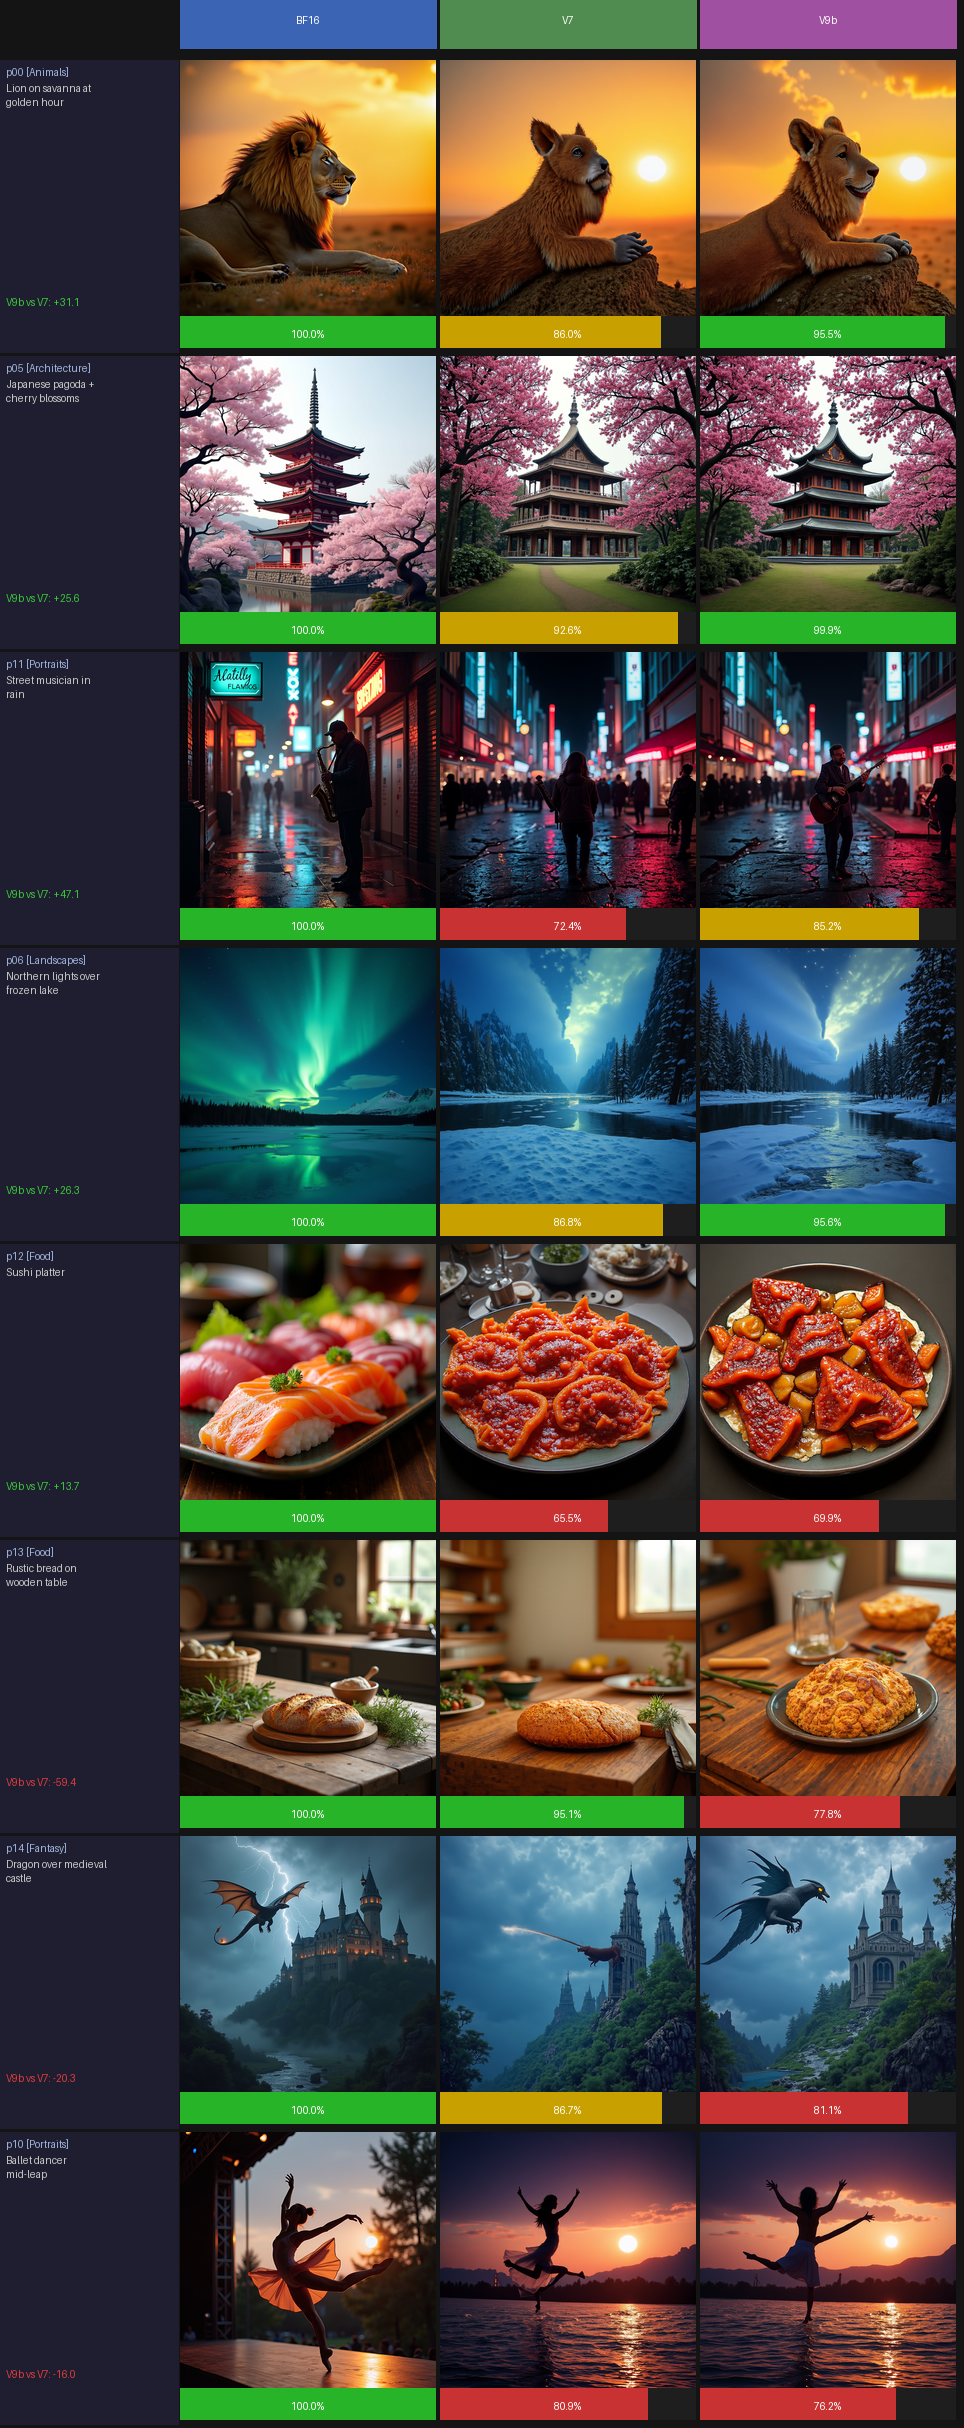
\includegraphics[width=0.75\textwidth]{figures/v9b_highlights.png}
  \caption{V9b (rank-64, 2{,}132 prompts) highlights: BF16 $|$ V7 $|$ V9b comparison for 8 selected prompts.}
  \label{fig:v9b_highlights}
\end{figure}

\end{document}
